\documentclass[12pt]{article}
\usepackage{amsmath, amssymb, graphicx, xcolor}
\usepackage{geometry}
\usepackage{placeins}
\geometry{margin=1in}

% Title and authors
\title{Gene Expression Analysis: Differentially Expressed Genes by Sex and Brain Region}
\author{Jia Guo, Feifan Jiang, Judy Wu}
\date{\today}

\begin{document}

\maketitle

\tableofcontents
\newpage

%%%%%%%%%%%% 1 %%%%%%%%%%%%
\section{Introduction}
Our dataset includes 84 samples collected from 10 patients after quality control checks. Each sample is annotated with metadata, including their sex, the brain region from which the sample was taken, the laboratory source, and the chip version used for measurement.

In our analysis, the log-transformed expression intensity data is included for 12600 genes. Each gene is represented by its symbol and chromosome location, though 892 genes have missing identity information, which may serve as controls. 

The goal of this analysis is to identify genes with significant differences in expression by sex (male and female) and by two brain regions (anterior cingulate cortex and dorsolateral prefrontal cortex). Due to the high cost of subsequent confirmatory studies, we will select not more than 20 genes for further investigation. These genes will be prioritized based on a confidence ranking, helping to focus future studies on the most promising candidates for differential expression.

%%%%%%%%%%%% 2 %%%%%%%%%%%%
\section{Exploratory Data Analysis \& Data Preparation}


To begin our analysis, we acknowledge that the dataset has already been through quality control checks. As a result, all 84 samples are included, and no additional exclusions will be made. Furthermore, we will retain all genes for analysis, even those without complete symbol or chromosome information, to ensure a thorough examination of all potential candidates.

\subsection{Data Overview}
    \subsubsection{Distribution of Gene Expression}
Next, we examine the distribution of gene expression levels across laboratory source and chip version to better understand the dataset. Figure~\ref{fig:original_data} displays these distributions together, highlighting the differences between the three laboratories, UC Davis, Michigan, and UC Irvine, as well as between the two chip versions. The expression levels differ notably across the labs, with UC Irvine showing relatively higher expression levels, Michigan having lower levels, and UC Davis displaying a middle expression level with a wider range of variance. 



\begin{figure}[h!]
    \centering
    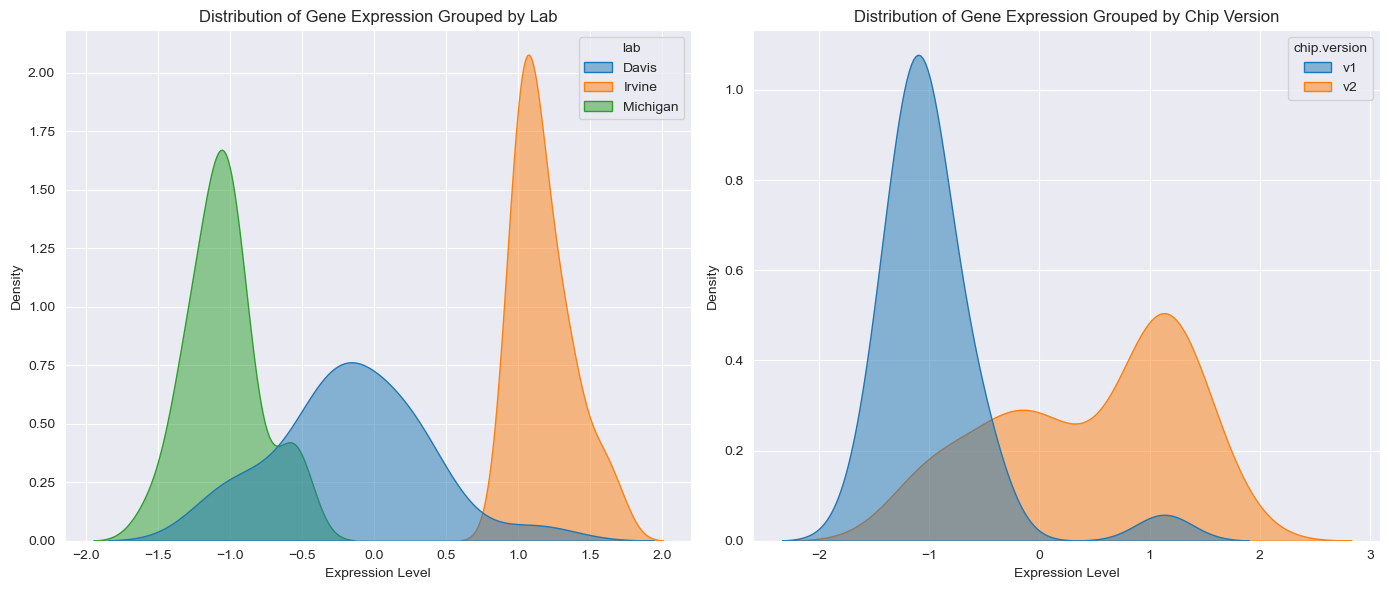
\includegraphics[width=.8\textwidth]{image/original_data}
    \caption{Distribution of expression levels by lab source and chip version}
    \label{fig:original_data}
\end{figure}
\FloatBarrier

Similarly, the distribution of expression levels varies by chip version, with chip version 2 (HG U95Av2) tending to show higher expression levels than chip version 1 (HG U95A). These patterns suggest that both laboratory source and chip version are important factors influencing the expression data.

These initial observations underscore the need to account for laboratory source and chip version as potential confounders in our analysis. The differences between the labs and chip versions suggest the presence of batch effects, which we will address in the following steps. 


\subsubsection{Consideration of Y Chromosome Genes}

To ensure a comprehensive analysis of sex-related differences in gene expression, we examined the distribution of Y chromosome genes across both sexes (Figure~\ref{fig:Y genes}). We observed that all selected Y chromosome genes exhibit measurable expression in both sexes, with just some showing slightly higher levels in males.

\begin{figure}[h!]
    \centering
    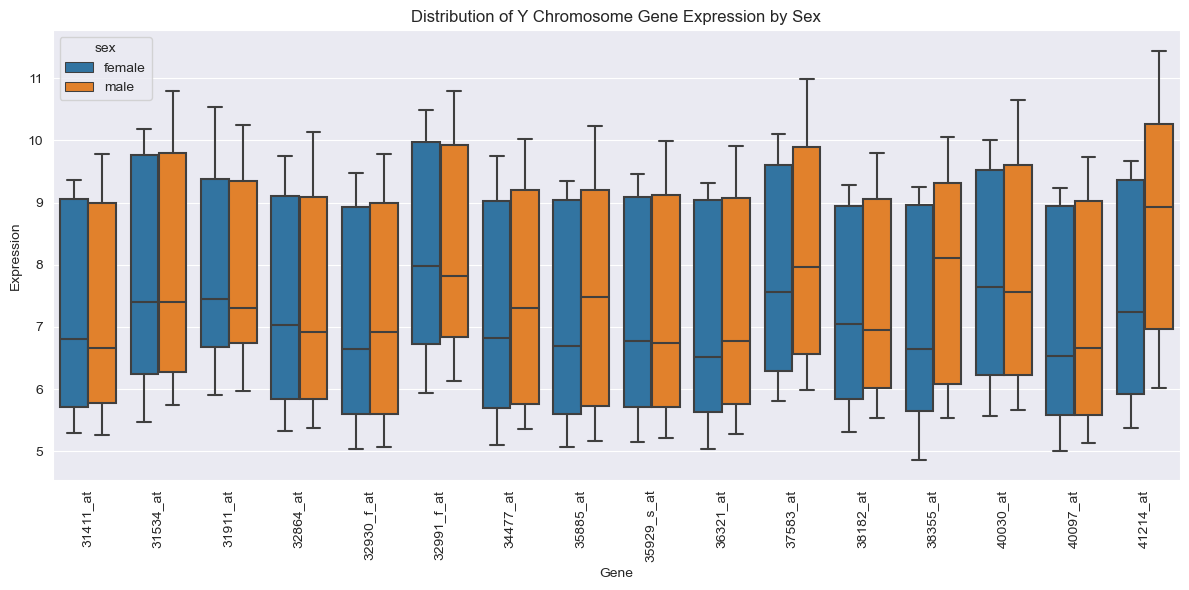
\includegraphics[width=.8\textwidth]{image/Y_gene_dist.png}
    \caption{Distribution of Y Chromosome Gene Expression by Sex}
    \label{fig:Y genes}
\end{figure}
\FloatBarrier

So in our analysis, we opted to retain Y chromosome genes. By keeping these Y chromosome genes, we can explore potential biological roles that they might play across both sexes, rather than dismissing them based solely on their chromosomal location.

Additionally, excluding these genes could result in missing important information about sex-specific gene interactions and functions. By keeping these genes, we ensure that we capture a more complete picture of gene expression differences, including the roles Y chromosome genes may play in both sexes.




\subsection{Data Preparation}

In this section, we apply a two-step data preparation using $Z$-Score normalization and Combat batch effect correction methods to prepare the gene expression data. Each method serves a distinct purpose in ensuring that the data is properly adjusted for biological comparison and free of technical bias.

In our study, we utilized two datasets, the \textit{normalized data} (the $Z$-Score normalized data) and the \textit{corrected data }(the normalized data with another layer of Combat correction). Based on the characteristics of each method, we used the \textit{corrected data} in T-test study and the \textit{normalized data} in GLM and Random Forest.



\subsubsection{Z-Score Normalization}

Z-Score normalization is used first to standardize the expression values across all samples, ensuring that each gene's expression levels are on the same scale. This method transforms the data so that each gene has a mean of zero and a standard deviation of one. The transformation is represented by the following equation:

\[
Z = \frac{x - \mu}{\sigma}
\]

Here, $x$ represents the raw or log-transformed expression value for a given gene, $\mu$ is the mean expression value of that gene across all samples, and $\sigma$ is the standard deviation. By applying Z-Score normalization, we ensure that the expression levels of all genes are standardized and comparable across the dataset.

\subsubsection{Combat Batch Effect Correction (for T-test)}

Combat batch effect correction is used after normalization to adjust for non-biological variability in the data that can result from differences in experimental conditions, such as the laboratory where the sample was processed or the chip version used. These batch effects introduce unwanted variation that may obscure the true biological differences we are interested in.  The Combat corrected data is used specifically in T-test analysis in our study to reduce the effect of inconsistency of gene expression between labs and chip versions. The details will be introduced in later section.

Combat uses an empirical Bayes framework to model and correct these batch effects, adjusting the data while preserving the biological signal of interest. The model used by Combat is described as:

\[
Y_{ij} = \alpha_i + \beta_j + \epsilon_{ij}
\]

In this model, $Y_{ij}$ represents the expression value of gene $i$ in sample $j$, $\alpha_i$ is the gene-specific effect, $\beta_j$ represents the batch effect (such as differences across labs or chip versions), and $\epsilon_{ij}$ is the residual noise. Combat estimates the batch effect $\beta_j$ and removes its influence from the expression data. This ensures that any observed differences in gene expression are due to biological factors, rather than technical artifacts.

\subsection{Data Preparation Results}

In this section, we compare the data structure before and after applying the batch correction using Combat. We visualize these changes through both direct distribution plots and Principal Component Analysis (PCA) to assess the effectiveness of the correction.

First, we examine the distribution of the corrected data by laboratory and chip version. Figure~\ref{fig:batch_correction} shows the distribution of the data points for the corrected dataset, grouped by lab and by chip version. After the batch correction, there is a significant overlap in the distribution of data points across the three labs and two chip versions, indicating that the method effectively mitigated the batch effect. The distinction between the different labs and chip versions is greatly reduced, resulting in a more homogeneous dataset.

\begin{figure}[h!]
    \centering
    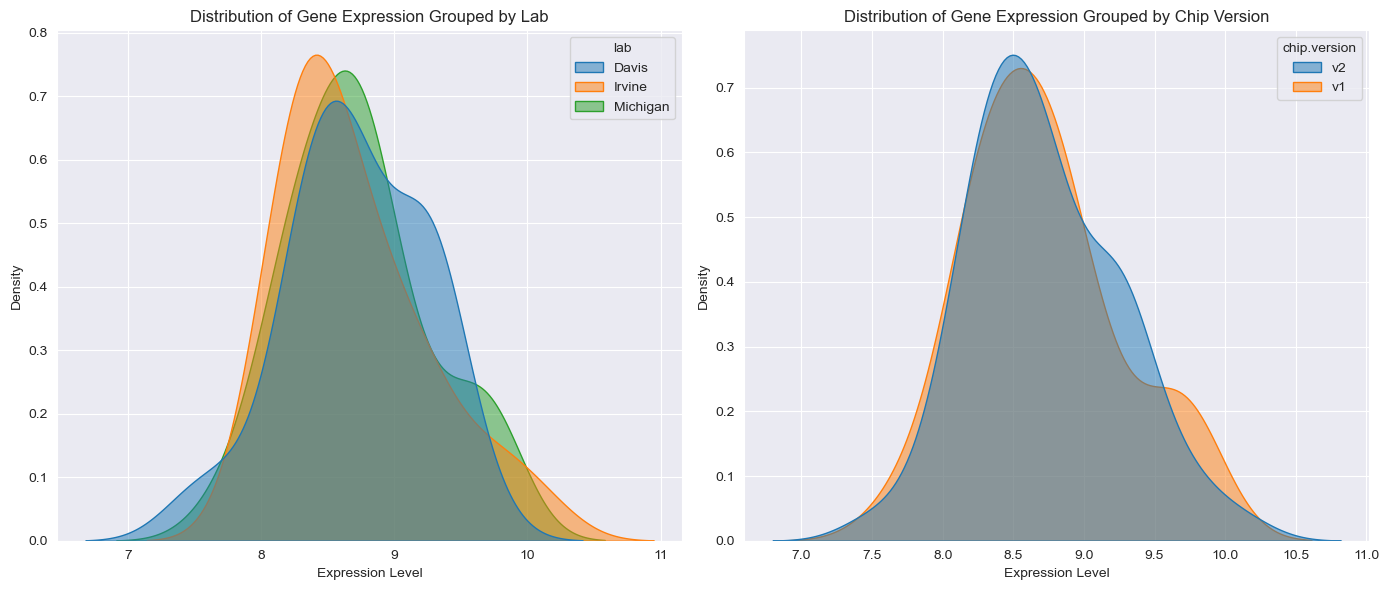
\includegraphics[width=0.8\textwidth]{image/batch_correction}
    \caption{Distribution of expression levels by lab and chip version after batch correction}
    \label{fig:batch_correction}
\end{figure}
\FloatBarrier

To further demonstrate the effect of batch correction, we visualize the dataset using Principal Component Analysis (PCA). Figures~\ref{fig:PCA_lab} and \ref{fig:PCA_chip} illustrate the PCA structure of the data before and after correction. Both plots represent the same underlying PCA data structure, but one figure highlights the data points by laboratory source and the other by chip version. 

\begin{figure}[h!]
    \centering
    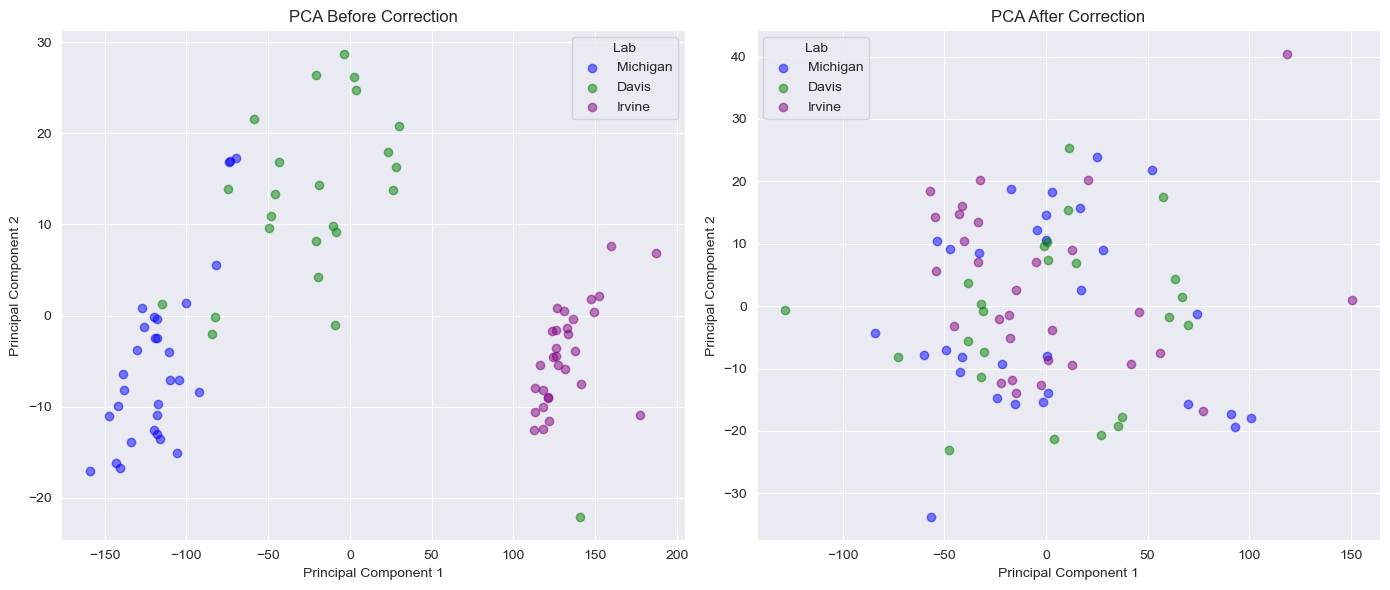
\includegraphics[width=0.8\textwidth]{image/PCA_lab}
    \caption{PCA plot labeled by laboratory source before and after batch correction}
    \label{fig:PCA_lab}
\end{figure}
\FloatBarrier

\begin{figure}[h!]
    \centering
    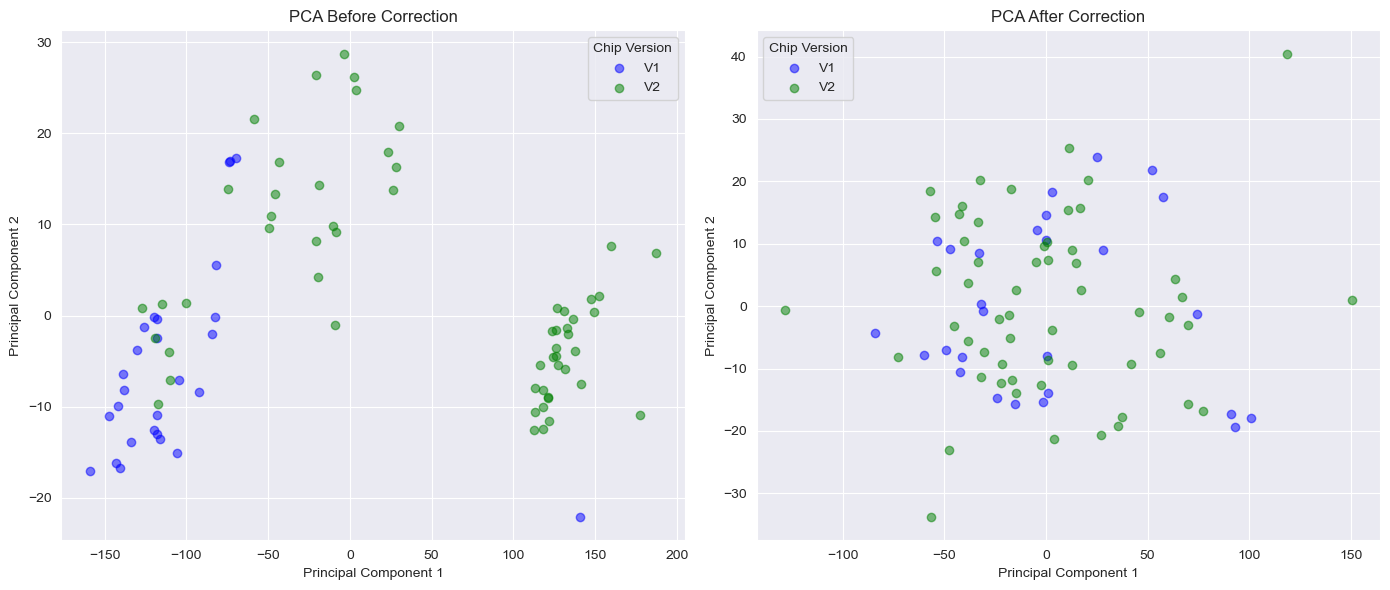
\includegraphics[width=0.8\textwidth]{image/PCA_chip}
    \caption{PCA plot labeled by chip version before batch correction}
    \label{fig:PCA_chip}
\end{figure}
\FloatBarrier

Before correction, clear clustering is visible based on laboratory source and chip version, suggesting that the batch effect is driving significant differences in the dataset. However, after batch correction, these clusters become less distinct, as evidenced by the mixture of data points from different labs and chip versions. This indicates that the batch effect has been successfully mitigated.

Additionally, when comparing the two PCA plots, we observe a large overlap between data points from the Michigan laboratory and those corresponding to chip version 1. This suggests that the Michigan lab predominantly used chip version 1 for its measurements.

In conclusion, the batch effect correction using Combat significantly reduced the influence of both laboratory source and chip versions on the data. By using the corrected data, we can analyze samples from different labs and chip versions together, eliminating the need to perform separate T-tests for each lab.


%%%%%%%%%%%% 3 %%%%%%%%%%%%
\section{Methods}
We will use multiple methods to analyze the data and detect significant differentially expressed genes. Below is an overview of the statistical models and algorithms used:

\subsection{T-test Analysis and T-test with Bootstrapping}

We apply Welch’s $t$-test to detect differentially expressed genes between sexes and brain regions. Welch’s $t$-test, which accounts for unequal variances between groups, calculates the test statistic as:

\[
t = \frac{\bar{x}_1 - \bar{x}_2}{\sqrt{\dfrac{s_1^2}{n_1} + \dfrac{s_2^2}{n_2}}}
\]

where $\bar{x}_1$ and $\bar{x}_2$ are the group means, $s_1^2$ and $s_2^2$ are the variances, and $n_1$ and $n_2$ are the sample sizes. $p$-values are adjusted to control for false discovery.

As a follow-up method, we apply bootstrapping by resampling the data 500 times. In each run, we perform Welch's $t$-test and select the top 50 genes based on adjusted p-values. Genes are ranked by how frequently they appear in the top 50 across iterations. The top five genes with the highest frequencies are reported for further investigation, offering a measure of consistency in differential expression across multiple resamples. This method allows us to further validate the results from initial t-test and recognize some genes that consistently show differential expressions even though they do not reach the statistical significance.

\subsection{Generalized Linear Model (GLM)}

We fit a Generalized Linear Model (GLM) to the normalized gene expression data without applying Combat batch effect correction. Instead, the model incorporates laboratory source and chip version as covariates to adjust for these variables. 

We apply Bonferroni correction with $\alpha = 0.05$ to control the family-wise error rate, and we report genes with a corrected $p$-value below 0.05 as significant.


\subsection{Random Forest Analysis}

We applied a Random Forest model to the normalized gene expression data, treating laboratory source and chip version as dummy variables to adjust for batch effects. The Random Forest algorithm uses an ensemble of decision trees to rank the importance of genes based on Gini importance, which measures the contribution of each gene to reducing impurity in the trees. Cross-validation was employed to minimize the risk of overfitting, ensuring the stability of the feature rankings. Genes with the top 5 Gini importance were identified as key candidates for further biological interpretation.

\subsection{Bayesian Modeling}

In this Bayesian approach, we aim to estimate the group mean $\theta$ and group covariance matrix $\Sigma$ for the two independent groups: either male versus female or the anterior cingulate cortex versus dorsolateral prefrontal cortex. We assume no interaction between groups and model each group using a multivariate normal distribution. For each group, we assume the prior for $\theta$ follows a normal distribution $\theta \sim N(\mu_0, \Sigma_0)$, and $\Sigma$ follows an inverse-Wishart distribution $\Sigma \sim \text{Inverse-Wishart}(\nu_0, S_0^{-1})$.

To update the posterior distribution of the parameters, we use Gibbs sampling. The conditional posterior for $\theta$ is a normal distribution, given by:

\[
\theta | Y, \Sigma \sim N\left( \left(\Sigma_0^{-1} + n\Sigma^{-1}\right)^{-1}\left(\Sigma_0^{-1}\mu_0 + n\Sigma^{-1} \bar{Y}\right), \left(\Sigma_0^{-1} + n\Sigma^{-1}\right)^{-1} \right),
\]

where $\bar{Y}$ is the mean of the observed data, and $n$ is the sample size. The posterior for $\Sigma$ is updated using an inverse-Wishart distribution:

\[
\Sigma | Y, \theta \sim \text{Inverse-Wishart}(\nu_0 + n, S_0 + \sum_{i=1}^{n}(Y_i - \theta)(Y_i - \theta)^T),
\]

where $\nu_0$ is the degrees of freedom, and $S_0$ is the scale matrix. We run 1100 iterations of the Gibbs sampler, discarding the first 100 as burn-in, to estimate the posterior distributions of the group means and covariance matrices.

To reduce the computational burden, we limit our analysis to genes identified as significant in previous steps, including $t$-tests, Random Forest, and GLM results. We calculate the difference between the posterior means of the two groups and rank the genes based on the magnitude of this difference. The top five genes with the largest differences are reported as the most differentially expressed. We also visualize the posterior covariance matrix to understand the relationships between the selected genes.

%%%%%%%%%%%% 4 %%%%%%%%%%%%
\section{Results}

In this section, we present the significant genes identified by each method, focusing on the comparison between male and female, and between the two brain regions (A.C. cortex and D.L.P.F. cortex).

\subsection{Significant Genes by T-test}

Using the batch effect corrected data, a standard $t$-test was performed to identify differentially expressed genes. For the comparison between male and female, two genes were found to be significantly differentially expressed. The table below summarizes these genes along with their adjusted p-values.

\begin{table}[h!]
\centering
\begin{tabular}{|c|c|c|c|}
\hline
\textbf{Gene Name} & \textbf{Symbol} & \textbf{Chromosome} & \textbf{Adjusted p-value} \\
\hline
41214\_at & RPS4Y1 & Y & $2.4 \times 10^{-13}$ \\
38355\_at & DDX3Y & Y & $2.4 \times 10^{-9}$ \\
\hline
\end{tabular}
\caption{Significant differentially expressed genes between male and female from $t$-test}
\end{table}

However, no significant differentially expressed genes were found between the two brain regions (A.C. cortex and D.L.P.F. cortex) using the standard $t$-test. Therefore, it became necessary to apply the bootstrap technique to further explore potential differences. By resampling 500 times, we ranked the genes by their frequency of appearance in the top 50 significant genes in each iteration.

Below, the top five genes ranked by frequency for the comparison between male and female are shown:

\begin{table}[h!]
\centering
\begin{tabular}{|c|c|c|c|}
\hline
\textbf{Gene Name} & \textbf{Symbol} & \textbf{Chromosome} & \textbf{Frequency} \\
\hline
41214\_at & RPS4Y1 & Y & 1.000 \\
38355\_at & DDX3Y & Y & 1.000 \\
37583\_at & KDM5D & Y & 0.688 \\
35885\_at & USP9Y & Y & 0.658 \\
1000\_at & MAPK3 & 16 & 0.556 \\
\hline
\end{tabular}
\caption{Top 5 differentially expressed genes between male and female by Bootstrap}
\end{table}

The bootstrap analysis for the sex problem revealed a high degree of overlap with the standard $t$-test results. The top two genes identified by the $t$-test, RPS4Y1 and DDX3Y, were also consistently selected in 100\% of the bootstrap iterations, further validating their significance as differentially expressed between males and females. The additional genes identified through bootstrapping, such as KDM5D and USP9Y, provide supplementary evidence for other potential candidates that may not have reached statistical significance in the original test but demonstrate consistent differential expression across resampling.

For the comparison between A.C. cortex and D.L.P.F. cortex, the top five genes ranked by frequency from the bootstrap resampling are presented in the following table:

\begin{table}[h!]
\centering
\begin{tabular}{|c|c|c|c|}
\hline
\textbf{Gene Name} & \textbf{Symbol} & \textbf{Chromosome} & \textbf{Frequency} \\
\hline
37134\_f\_at & GRIN1 & 9 & 0.602 \\
37135\_f\_at & GRIN1 & 9 & 0.484 \\
34500\_at & CABP1 & 12 & 0.420 \\
36150\_at & PLEKHM2 & 1 & 0.404 \\
38516\_at & SCN1B & 19 & 0.380 \\
\hline
\end{tabular}
\caption{Top 5 differentially expressed genes between A.C. cortex and D.L.P.F. cortex by Bootstrap}
\end{table}

In contrast to the sex analysis, although the top-ranked genes were identified, the results from the bootstrap analysis were not ideal. The highest gene appearance frequency was only around 60\%, indicating a lack of consistency in identifying these genes as differentially expressed across the two brain regions. Rather than viewing these findings as definitive, we recommend using them as a reference for future investigations.

\subsection{Significant Genes by GLM}

The Generalized Linear Model (GLM) was applied to the normalized data, accounting for potential batch effects by including laboratory source and chip version as covariates. Two genes were found to be significantly differentially expressed between male and female, as shown in the table below:

\begin{table}[h!]
\centering
\begin{tabular}{|c|c|c|c|}
\hline
\textbf{Gene Name} & \textbf{Symbol} & \textbf{Chromosome} & \textbf{Adjusted p-value} \\
\hline
41214\_at & RPS4Y1 & Y & $2.5 \times 10^{-26}$ \\
38355\_at & DDX3Y & Y & $1.6 \times 10^{-14}$ \\
\hline
\end{tabular}
\caption{Significant differentially expressed genes between male and female from GLM}
\end{table}

These two genes, RPS4Y1 and DDX3Y, were also identified by both the $t$-test and bootstrap methods, confirming their strong differential expression between male and female groups.

For the comparison between A.C. cortex and D.L.P.F. cortex, one gene was found to be significantly differentially expressed, as presented below:

\begin{table}[h!]
\centering
\begin{tabular}{|c|c|c|c|}
\hline
\textbf{Gene Name} & \textbf{Symbol} & \textbf{Chromosome} & \textbf{Adjusted p-value} \\
\hline
35457\_at & CARTPT & 5 & $0.021$ \\
\hline
\end{tabular}
\caption{Significant differentially expressed gene between A.C. cortex and D.L.P.F. cortex from GLM}
\end{table}

In contrast to the $t$-test, which did not identify any significant genes between the brain regions, GLM detected CARTPT as a differentially expressed gene. This suggests that including batch effect covariates may provide additional sensitivity in detecting expression differences between brain regions.

\subsection{Significant Genes by Random Forest}

Using the Random Forest model, we ranked genes based on their Gini importance, which measures each gene’s contribution to reducing impurity in the classification trees. The table below presents the top 5 genes identified based on their Gini importance for the comparison between male and female:

\begin{table}[h!]
\centering
\begin{tabular}{|c|c|c|c|}
\hline
\textbf{Gene Name} & \textbf{Symbol} & \textbf{Chromosome} & \textbf{Gini Importance} \\
\hline
41214\_at & RPS4Y1 & Y & 0.0103 \\
38355\_at & DDX3Y & Y & 0.0075 \\
35680\_r\_at & DPP6 & 7 & 0.0032 \\
31687\_f\_at & HBB & 11 & 0.0031 \\
38446\_at & XIST & X & 0.0028 \\
\hline
\end{tabular}
\caption{Top 5 genes ranked by Gini importance for male vs. female from Random Forest}
\end{table}

Similarly, the top 5 genes ranked by Gini importance for the comparison between A.C. cortex and D.L.P.F. cortex are shown in the table below:

\begin{table}[h!]
\centering
\begin{tabular}{|c|c|c|c|}
\hline
\textbf{Gene Name} & \textbf{Symbol} & \textbf{Chromosome} & \textbf{Gini Importance} \\
\hline
396\_f\_at & EPOR & 19 & 0.0044 \\
39854\_r\_at & PNPLA2 & 11 & 0.0034 \\
1826\_at & RHOB & 2 & 0.0029 \\
33903\_at & DAPK3 & 19 & 0.0025 \\
31957\_r\_at & RPLP1 & 15 & 0.0024 \\
\hline
\end{tabular}
\caption{Top 5 genes ranked by Gini importance for A.C. cortex vs. D.L.P.F. cortex from Random Forest}
\end{table}

The results from the Random Forest analysis show notable overlap with the previous methods for the comparison between male and female. Specifically, the genes RPS4Y1 and DDX3Y, which were identified as significant in both the $t$-test and GLM methods, also ranked highest in terms of Gini importance. This consistent identification across multiple methods strengthens the evidence for these genes' differential expression between sexes.

In contrast, the Random Forest analysis for the brain region comparison revealed no overlap with the results from the GLM or bootstrap methods. The top genes identified here, such as EPOR and PNPLA2, were not previously highlighted by the other methods. This lack of overlap could suggest that the Random Forest model is capturing a different aspect of the data, or that the brain region differences are more subtle and detected differently depending on the model used. Further investigation into these genes may be necessary to understand their role in brain region-specific expression.

\subsection{Significant Genes by Bayesian Modeling}

For the Bayesian modeling, we focused on a subset of genes identified as candidates from previous methods. Specifically, we analyzed 8 candidate genes for the male vs. female comparison and 11 candidate genes for the A.C. cortex vs. D.L.P.F. cortex comparison. The tables below present the top 5 genes from each comparison, ranked by the difference in their posterior means.

\textbf{Top 5 genes for male vs. female comparison:}

\begin{table}[h!]
\centering
\begin{tabular}{|c|c|c|c|}
\hline
\textbf{Gene Name} & \textbf{Symbol} & \textbf{Chromosome} & \textbf{Mean Difference} \\
\hline
41214\_at & RPS4Y1 & Y & 1.265 \\
38355\_at & DDX3Y & Y & 0.868 \\
31687\_f\_at & HBB & 11 & 0.572 \\
37583\_at & KDM5D & Y & 0.420 \\
35885\_at & USP9Y & Y & 0.376 \\
\hline
\end{tabular}
\caption{Top 5 genes ranked by mean difference for male vs. female from Bayesian modeling}
\end{table}

\textbf{Top 5 genes for A.C. cortex vs. D.L.P.F. cortex comparison:}

\begin{table}[h!]
\centering
\begin{tabular}{|c|c|c|c|}
\hline
\textbf{Gene Name} & \textbf{Symbol} & \textbf{Chromosome} & \textbf{Mean Difference} \\
\hline
34500\_at & CABP1 & 12 & 1.013 \\
37135\_f\_at & GRIN1 & 9 & 0.477 \\
31957\_r\_at & RPLP1 & 15 & 0.450 \\
37134\_f\_at & GRIN1 & 9 & 0.410 \\
38516\_at & SCN1B & 19 & 0.293 \\
\hline
\end{tabular}
\caption{Top 5 genes ranked by mean difference for A.C. cortex vs. D.L.P.F. cortex from Bayesian modeling}
\end{table}

In this confirmation study, Bayesian modeling reaffirms several of the previously identified significant genes from other methods. For the male vs. female comparison, RPS4Y1 and DDX3Y continue to show large mean differences, further validating their differential expression. HBB, which appears on chromosome 11, also exhibits a noticeable difference, indicating its potential role in the biological processes.

Next, we visualize the posterior covariance matrices for the male and female groups, and for the A.C. cortex and D.L.P.F. cortex groups. The posterior covariance matrices allow us to observe the relationships between the selected genes in each group.

\begin{figure}[h!]
    \centering
    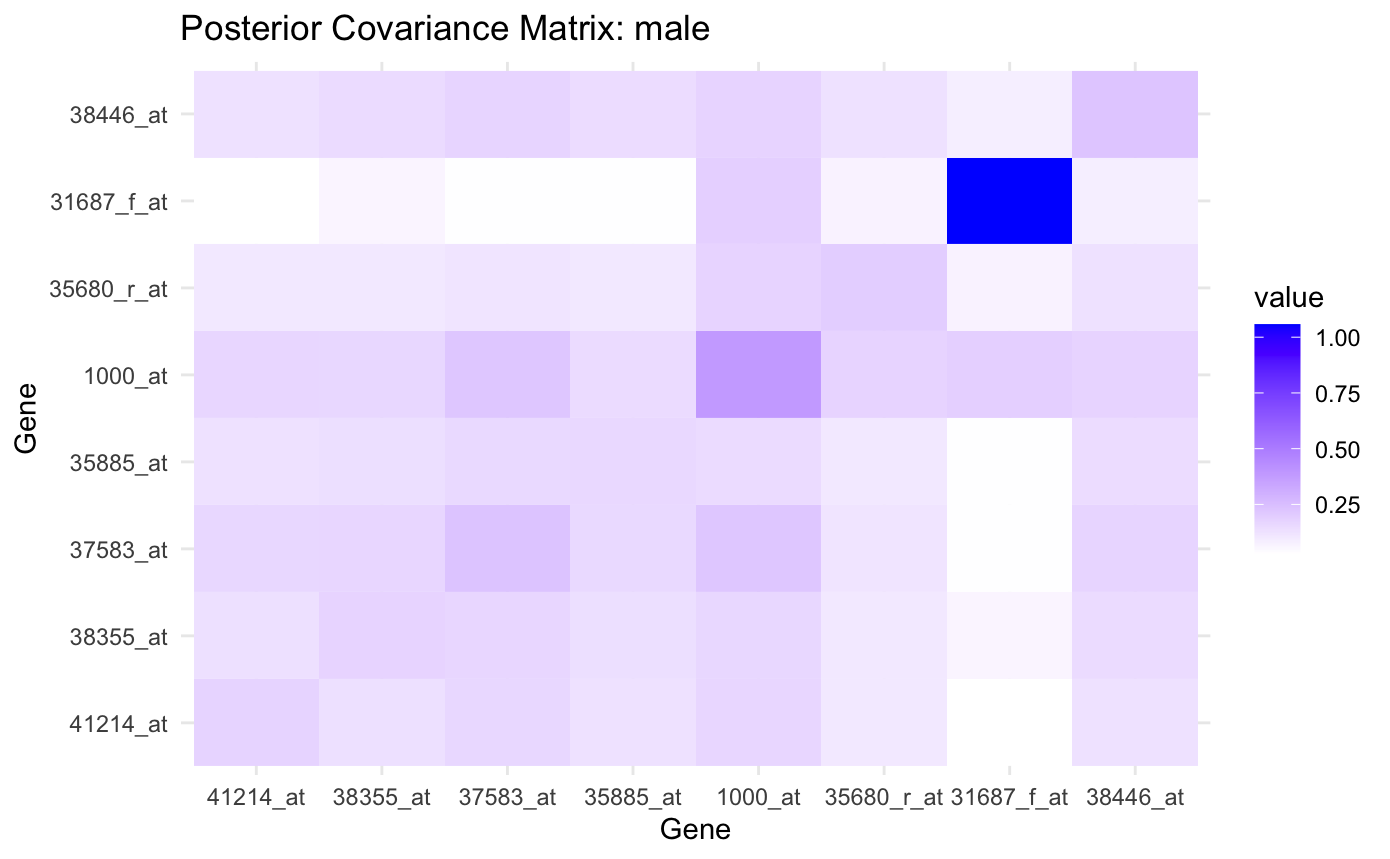
\includegraphics[width=0.45\textwidth]{image/pos_cov_male}
    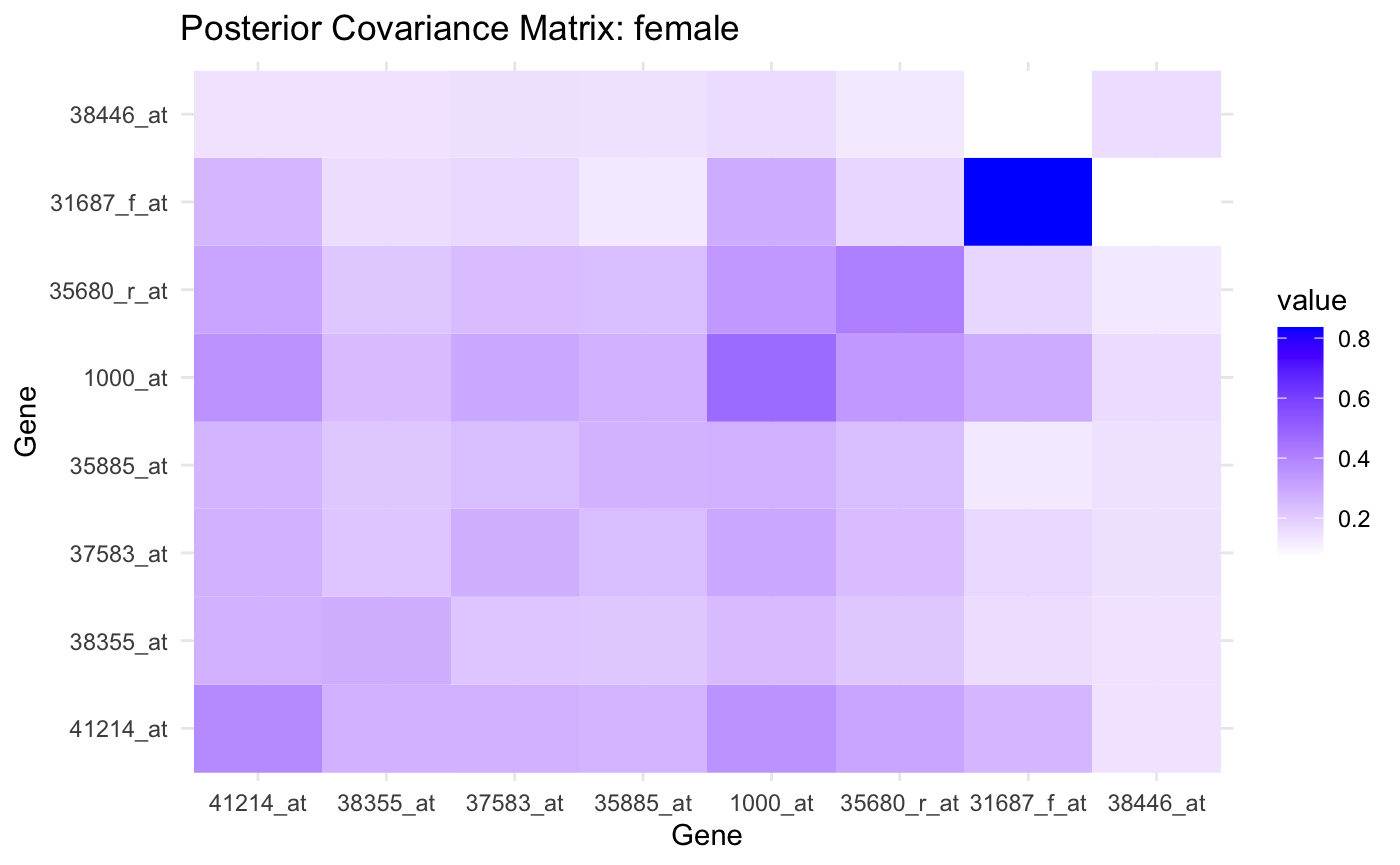
\includegraphics[width=0.45\textwidth]{image/pos_cov_female}
    \caption{Posterior covariance matrix for male (left) and female (right)}
    \label{fig:cov_male_female}
\end{figure}
\FloatBarrier

The covariance matrices for male and female groups reveal some key differences. In the male group, HBB, located on chromosome 11, exhibits nearly zero covariance with other genes. In contrast, in the female group, HBB shows higher covariance with other genes, suggesting potential interactions or regulatory effects that differ between the sexes.

\begin{figure}[h!]
    \centering
    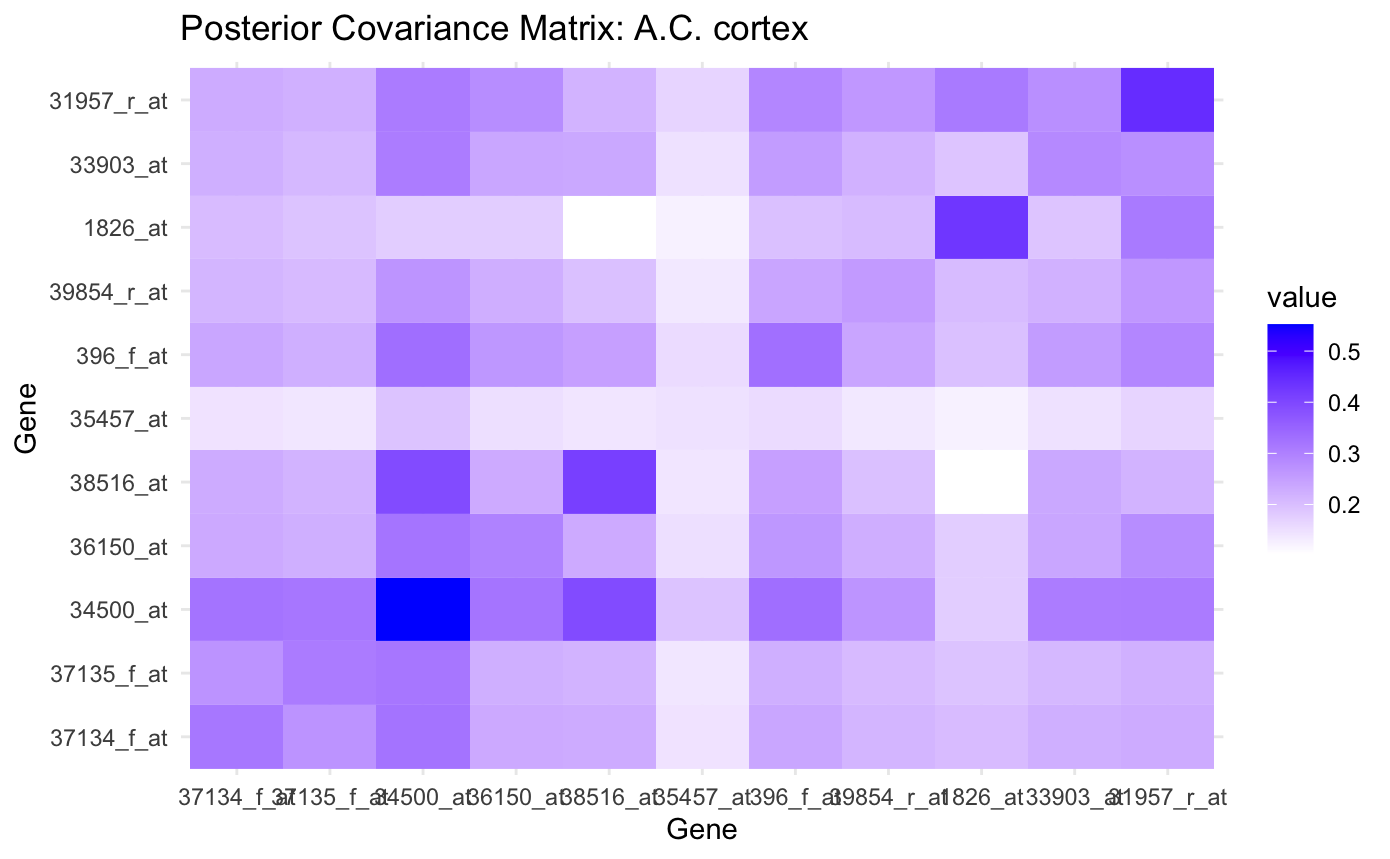
\includegraphics[width=0.45\textwidth]{image/pos_cov_AC}
    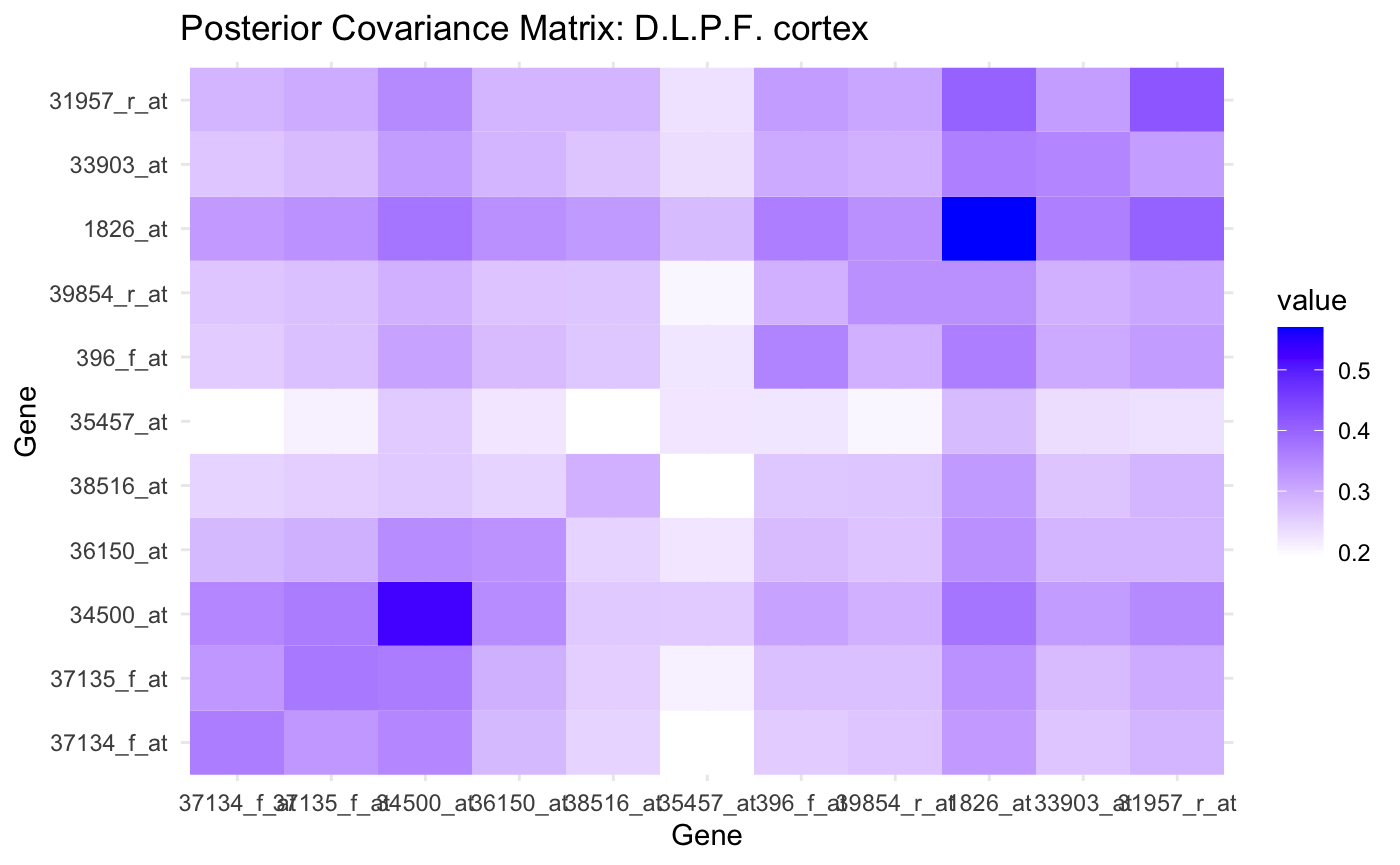
\includegraphics[width=0.45\textwidth]{image/pos_cov_DLPF}
    \caption{Posterior covariance matrix for A.C. cortex (left) and D.L.P.F. cortex (right)}
    \label{fig:cov_AC_DLPF}
\end{figure}
\FloatBarrier

For the A.C. cortex and D.L.P.F. cortex comparison, the covariance matrices show distinct patterns. Genes such as CABP1 and GRIN1 exhibit stronger covariance in one brain region over the other, suggesting that these genes might play region-specific roles in brain function. The differences in covariance patterns between A.C. cortex and D.L.P.F. cortex provide further evidence of brain region-specific gene expression, which may underlie functional differences between these areas.

In summary, the Bayesian modeling results confirm the differential expression of key genes identified in previous methods and provide deeper insight into the covariance structures, offering clues to the complex interactions between these genes within each group.

%%%%%%%%%%%% 5 %%%%%%%%%%%%
\section{Conclusion}
In this section, we summarize the findings from the different statistical and machine learning methods, presenting a confidence stratification of the identified genes for both the male vs. female comparison and the A.C. cortex vs. D.L.P.F. cortex comparison.

\begin{table}[h!]
\centering
\begin{tabular}{|c|c|c|c|c|}
\hline
\textbf{Name} & \textbf{Symbol} & \textbf{Chromosome} & \textbf{Tests} & \textbf{Confidence} \\
\hline
41214\_at & RPS4Y1 & Y & T-test, Boots, GLM, RF, Bayes & High \\
38355\_at & DDX3Y & Y & T-test, Boots, GLM, RF, Bayes & High \\
35885\_at & USP9Y & Y & Boots, Bayes & Medium \\
37583\_at & KDM5D & Y & Boots, Bayes & Medium \\
31687\_f\_at & HBB & 11 & RF, Bayes& Medium \\
35680\_r\_at & DPP6 & 7 & RF & Low \\
38446\_at & XIST & X & RF & Low \\
1000\_at & MAPK3 & 16 & Boots & Low \\
\hline
\end{tabular}
\caption{Confidence stratification for male vs. female comparison}
\end{table}

\begin{table}[h!]
\centering
\begin{tabular}{|c|c|c|c|c|}
\hline
\textbf{Name} & \textbf{Symbol} & \textbf{Chromosome} & \textbf{Tests} & \textbf{Confidence} \\
\hline
37134\_f\_at & GRIN1 & 9 & Boots, Bayes & Medium \\
37135\_f\_at & GRIN1 & 9 & Boots, Bayes & Medium \\
34500\_at & CABP1 & 12 & Boots, Bayes & Medium \\
38516\_at & SCN1B & 19 & Boots, Bayes & Medium \\
31957\_r\_at & RPLP1 & 15 & RF, Bayes & Medium \\
36150\_at & PLEKHM2 & 1 & Boots & Low \\
396\_f\_at & EPOR & 19 & RF & Low \\
39854\_r\_at & PNPLA2 & 11 & RF & Low \\
1826\_at & RHOB & 2 & RF & Low \\
33903\_at & DAPK3 & 19 & RF & Low \\
35457\_at & CARTPT & 5 & GLM & Low \\
\hline
\end{tabular}
\caption{Confidence stratification for A.C. cortex vs. D.L.P.F. cortex comparison}
\end{table}


For the male vs. female comparison, we highly recommend further investigation of the high-confidence genes, RPS4Y1 and DDX3Y, as they were consistently significant across all methods, indicating strong evidence of differential expression. Medium-confidence genes, such as USP9Y and KDM5D, also warrant additional investigation due to their consistent identification in bootstrap and Bayesian methods. However, the low-confidence genes identified by only one or two methods, such as DPP6 and MAPK3, are not recommended for immediate focus without further supporting evidence.




For the A.C. cortex vs. D.L.P.F. cortex comparison, none of the identified genes achieved high confidence, indicating that additional evidence is needed to support strong conclusions about differential expression in these brain regions. However, we suggest a thorough but cautious investigation of the medium-confidence genes, such as GRIN1 and CABP1, which were identified across multiple methods, making them the most promising candidates. Some of the low-confidence genes, like EPOR and CARTPT, may also merit further exploration given their identification in specific models, but they should be approached with care due to their limited evidence.


\end{document}

